%% vc.tex %%
  \subsection{Présentation de l'algorithme}
  \begin{frame}
   \frametitle{Algorithme}
   \begin{block}{Idée}
    \begin{itemize}
     \item Méthode: Parcours en profondeur
     \item Aller: Marquer les pères d'au moins une feuille
     \item Retour: Marquer les sommets pères de sommets non marqués
    \end{itemize}
   \end{block}

   \begin{block}{Complexité}
    La complexité est celle du parcours en profondeur : $O(|V| + |E|)$.
   \end{block}
  \end{frame}

  \subsection{Exemple d'exécution}
  \begin{frame}
   \frametitle{Exécution}

   \begin{block}{\only<-19>{Application de l'algorithme}\only<20->{Solution}}
    \begin{center}
     \begin{figure}[!ht]
      \only<1>{
      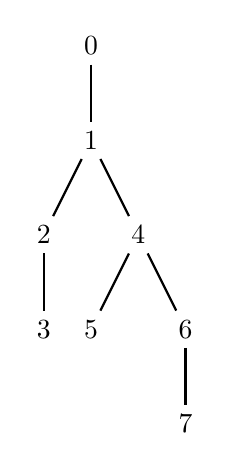
\begin{tikzpicture}
       \tikzstyle{level 1}=[level distance=1.2cm, sibling distance=1.2cm]
       \tikzstyle{childnode}=[rounded corners]
       \tikzstyle{marknode}=[fill=red!30, rounded corners]
       \tikzstyle{edge from parent}=[draw,thick]
       \node% [fill=red!30]
       {0} 
        child {node[childnode] {1} 
         child {node[childnode] {2}
          child {node[childnode] {3}
          }
         }
         child {node[childnode] {4}
          child {node[childnode] {5}
          }
          child {node[childnode] {6} 
           child {node[childnode] {7}}
          }
         }
        };
      \end{tikzpicture}
      }\only<2>{
      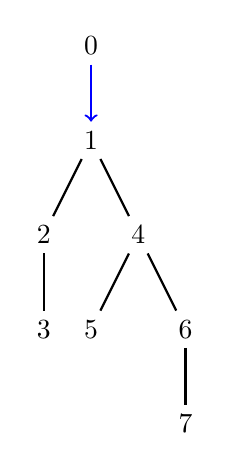
\begin{tikzpicture}
       \tikzstyle{level 1}=[level distance=1.2cm, sibling distance=1.2cm]
       \tikzstyle{childnode}=[rounded corners, black]
       \tikzstyle{marknode}=[fill=red!30, rounded corners]
       \tikzstyle{edge from parent}=[draw,thick]
       \node {0} 
        child[blue, ->] {node[childnode] {1} 
         child[black, -] {node[childnode] {2}
          child {node[childnode] {3}
          }
         }
         child[black, -] {node[childnode] {4}
          child {node[childnode] {5}
          }
          child {node[childnode] {6} 
           child {node[childnode] {7}}
          }
         }
        };
      \end{tikzpicture}
      }\only<3>{
      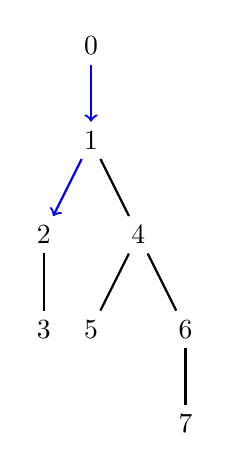
\begin{tikzpicture}
       \tikzstyle{level 1}=[level distance=1.2cm, sibling distance=1.2cm]
       \tikzstyle{childnode}=[rounded corners, black]
       \tikzstyle{marknode}=[fill=red!30, rounded corners]
       \tikzstyle{edge from parent}=[draw,thick]
       \node {0} 
        child[blue, ->] {node[childnode] {1} 
         child {node[childnode] {2}
          child[black, -] {node[childnode] {3}
          }
         }
         child[black, -] {node[childnode] {4}
          child {node[childnode] {5}
          }
          child {node[childnode] {6} 
           child {node[childnode] {7}}
          }
         }
        };
      \end{tikzpicture}
      }\only<4>{
      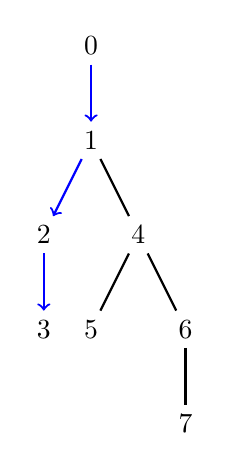
\begin{tikzpicture}
       \tikzstyle{level 1}=[level distance=1.2cm, sibling distance=1.2cm]
       \tikzstyle{childnode}=[rounded corners, black]
       \tikzstyle{marknode}=[fill=red!30, rounded corners]
       \tikzstyle{edge from parent}=[draw,thick]
       \node {0} 
        child[blue, ->] {node[childnode] {1} 
         child {node[childnode] {2}
          child {node[childnode] {3}
          }
         }
         child[black, -] {node[childnode] {4}
          child {node[childnode] {5}
          }
          child {node[childnode] {6} 
           child {node[childnode] {7}}
          }
         }
        };
      \end{tikzpicture}
      }\only<5>{
      \begin{tikzpicture}
       \tikzstyle{level 1}=[level distance=1.2cm, sibling distance=1.2cm]
       \tikzstyle{childnode}=[rounded corners, black]
       \tikzstyle{marknode}=[fill=red!30, rounded corners]
       \tikzstyle{edge from parent}=[draw,thick]
       \node {0} 
        child[blue, ->] {node[childnode] {1} 
         child {node[childnode] {2}
          child[red, <-] {node[childnode] {3}
           edge from parent node[left] {true}
          }
         }
         child[black, -] {node[childnode] {4}
          child {node[childnode] {5}
          }
          child {node[childnode] {6} 
           child {node[childnode] {7}}
          }
         }
        };
      \end{tikzpicture}
      }\only<6>{
      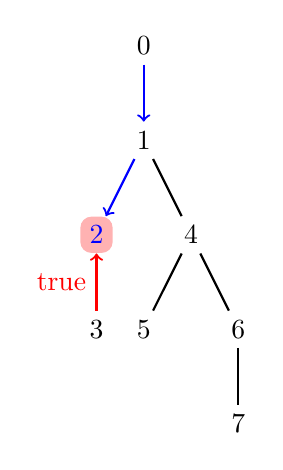
\begin{tikzpicture}
       \tikzstyle{level 1}=[level distance=1.2cm, sibling distance=1.2cm]
       \tikzstyle{childnode}=[rounded corners, black]
       \tikzstyle{marknode}=[fill=red!30, rounded corners]
       \tikzstyle{edge from parent}=[draw,thick]
       \node {0} 
        child[blue, ->] {node[childnode] {1} 
         child {node[marknode] {\Cb{2}}
          child[red, <-] {node[childnode] {3}
           edge from parent node[left] {true}
          }
         }
         child[black, -] {node[childnode] {4}
          child {node[childnode] {5}
          }
          child {node[childnode] {6} 
           child {node[childnode] {7}}
          }
         }
        };
      \end{tikzpicture}
      }\only<7>{
      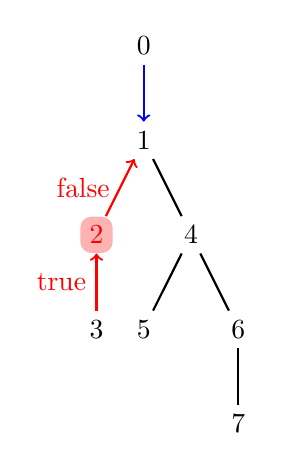
\begin{tikzpicture}
       \tikzstyle{level 1}=[level distance=1.2cm, sibling distance=1.2cm]
       \tikzstyle{childnode}=[rounded corners, black]
       \tikzstyle{marknode}=[fill=red!30, rounded corners]
       \tikzstyle{edge from parent}=[draw,thick]
       \node {0} 
        child[blue, ->] {node[childnode] {1} 
         child[red, <-] {node[marknode] {\Cb{2}}
          child {node[childnode] {3}
           edge from parent node[left] {true}
          }
          edge from parent node[left] {false}
         }
         child[black, -] {node[childnode] {4}
          child {node[childnode] {5}
          }
          child {node[childnode] {6} 
           child {node[childnode] {7}}
          }
         }
        };
      \end{tikzpicture}
      }\only<8>{
      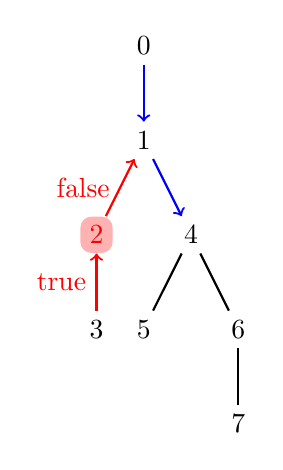
\begin{tikzpicture}
       \tikzstyle{level 1}=[level distance=1.2cm, sibling distance=1.2cm]
       \tikzstyle{childnode}=[rounded corners, black]
       \tikzstyle{marknode}=[fill=red!30, rounded corners]
       \tikzstyle{edge from parent}=[draw,thick]
       \node {0} 
        child[blue, ->] {node[childnode] {1} 
         child[red, <-] {node[marknode] {\Cb{2}}
          child {node[childnode] {3}
           edge from parent node[left] {true}
          }
          edge from parent node[left] {false}
         }
         child {node[childnode] {4}
          child[black, -] {node[childnode] {5}
          }
          child[black, -] {node[childnode] {6} 
           child {node[childnode] {7}}
          }
         }
        };
      \end{tikzpicture}
      }\only<9>{
      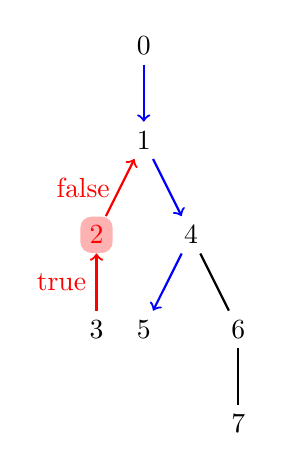
\begin{tikzpicture}
       \tikzstyle{level 1}=[level distance=1.2cm, sibling distance=1.2cm]
       \tikzstyle{childnode}=[rounded corners, black]
       \tikzstyle{marknode}=[fill=red!30, rounded corners]
       \tikzstyle{edge from parent}=[draw,thick]
       \node {0} 
        child[blue, ->] {node[childnode] {1} 
         child[red, <-] {node[marknode] {\Cb{2}}
          child {node[childnode] {3}
           edge from parent node[left] {true}
          }
          edge from parent node[left] {false}
         }
         child {node[childnode] {4}
          child {node[childnode] {5}
          }
          child[black, -] {node[childnode] {6} 
           child {node[childnode] {7}}
          }
         }
        };
      \end{tikzpicture}
      }\only<10>{
      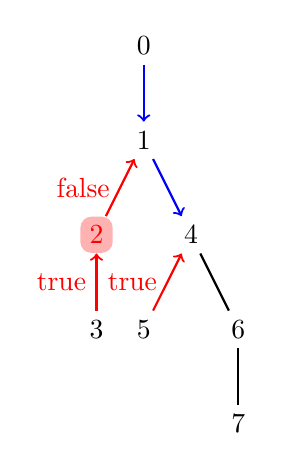
\begin{tikzpicture}
       \tikzstyle{level 1}=[level distance=1.2cm, sibling distance=1.2cm]
       \tikzstyle{childnode}=[rounded corners, black]
       \tikzstyle{marknode}=[fill=red!30, rounded corners]
       \tikzstyle{edge from parent}=[draw,thick]
       \node {0} 
        child[blue, ->] {node[childnode] {1} 
         child[red, <-] {node[marknode] {\Cb{2}}
          child {node[childnode] {3}
           edge from parent node[left] {true}
          }
          edge from parent node[left] {false}
         }
         child {node[childnode] {4}
          child[red, <-] {node[childnode] {5}
           edge from parent node[left] {true}
          }
          child[black, -] {node[childnode] {6} 
           child {node[childnode] {7}}
          }
         }
        };
      \end{tikzpicture}
      }\only<11>{
      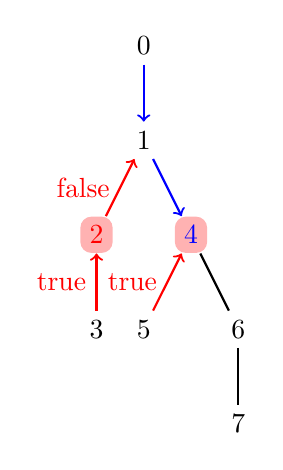
\begin{tikzpicture}
       \tikzstyle{level 1}=[level distance=1.2cm, sibling distance=1.2cm]
       \tikzstyle{childnode}=[rounded corners, black]
       \tikzstyle{marknode}=[fill=red!30, rounded corners]
       \tikzstyle{edge from parent}=[draw,thick]
       \node {0} 
        child[blue, ->] {node[childnode] {1} 
         child[red, <-] {node[marknode] {\Cb{2}}
          child {node[childnode] {3}
           edge from parent node[left] {true}
          }
          edge from parent node[left] {false}
         }
         child {node[marknode] {\Cb{4}}
          child[red, <-] {node[childnode] {5}
           edge from parent node[left] {true}
          }
          child[black, -] {node[childnode] {6} 
           child {node[childnode] {7}}
          }
         }
        };
      \end{tikzpicture}
      }\only<12>{
      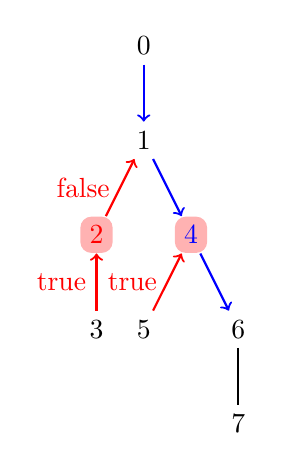
\begin{tikzpicture}
       \tikzstyle{level 1}=[level distance=1.2cm, sibling distance=1.2cm]
       \tikzstyle{childnode}=[rounded corners, black]
       \tikzstyle{marknode}=[fill=red!30, rounded corners]
       \tikzstyle{edge from parent}=[draw,thick]
       \node {0} 
        child[blue, ->] {node[childnode] {1} 
         child[red, <-] {node[marknode] {\Cb{2}}
          child {node[childnode] {3}
           edge from parent node[left] {true}
          }
          edge from parent node[left] {false}
         }
         child {node[marknode] {\Cb{4}}
          child[red, <-] {node[childnode] {5}
           edge from parent node[left] {true}
          }
          child {node[childnode] {6} 
           child[black, -] {node[childnode] {7}}
          }
         }
        };
      \end{tikzpicture}
      }\only<13>{
      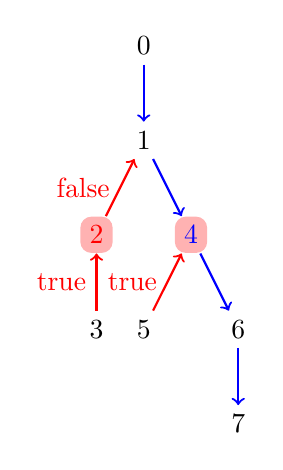
\begin{tikzpicture}
       \tikzstyle{level 1}=[level distance=1.2cm, sibling distance=1.2cm]
       \tikzstyle{childnode}=[rounded corners, black]
       \tikzstyle{marknode}=[fill=red!30, rounded corners]
       \tikzstyle{edge from parent}=[draw,thick]
       \node {0} 
        child[blue, ->] {node[childnode] {1} 
         child[red, <-] {node[marknode] {\Cb{2}}
          child {node[childnode] {3}
           edge from parent node[left] {true}
          }
          edge from parent node[left] {false}
         }
         child {node[marknode] {\Cb{4}}
          child[red, <-] {node[childnode] {5}
           edge from parent node[left] {true}
          }
          child {node[childnode] {6} 
           child {node[childnode] {7}}
          }
         }
        };
      \end{tikzpicture}
      }\only<14>{
      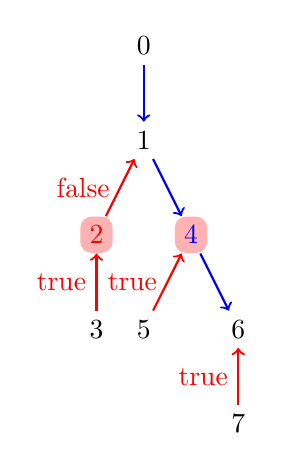
\begin{tikzpicture}
       \tikzstyle{level 1}=[level distance=1.2cm, sibling distance=1.2cm]
       \tikzstyle{childnode}=[rounded corners, black]
       \tikzstyle{marknode}=[fill=red!30, rounded corners]
       \tikzstyle{edge from parent}=[draw,thick]
       \node {0} 
        child[blue, ->] {node[childnode] {1} 
         child[red, <-] {node[marknode] {\Cb{2}}
          child {node[childnode] {3}
           edge from parent node[left] {true}
          }
          edge from parent node[left] {false}
         }
         child {node[marknode] {\Cb{4}}
          child[red, <-] {node[childnode] {5}
           edge from parent node[left] {true}
          }
          child {node[childnode] {6} 
           child[red, <-] {node[childnode] {7}
            edge from parent node[left] {true}
           }
          }
         }
        };
      \end{tikzpicture}
      }\only<15>{
      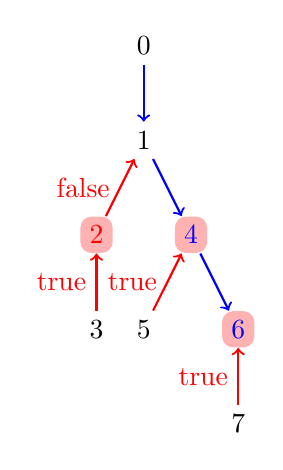
\begin{tikzpicture}
       \tikzstyle{level 1}=[level distance=1.2cm, sibling distance=1.2cm]
       \tikzstyle{childnode}=[rounded corners, black]
       \tikzstyle{marknode}=[fill=red!30, rounded corners]
       \tikzstyle{edge from parent}=[draw,thick]
       \node {0} 
        child[blue, ->] {node[childnode] {1} 
         child[red, <-] {node[marknode] {\Cb{2}}
          child {node[childnode] {3}
           edge from parent node[left] {true}
          }
          edge from parent node[left] {false}
         }
         child {node[marknode] {\Cb{4}}
          child[red, <-] {node[childnode] {5}
           edge from parent node[left] {true}
          }
          child {node[marknode] {\Cb{6}}
           child[red, <-] {node[childnode] {7}
            edge from parent node[left] {true}
           }
          }
         }
        };
      \end{tikzpicture}
      }\only<16>{
      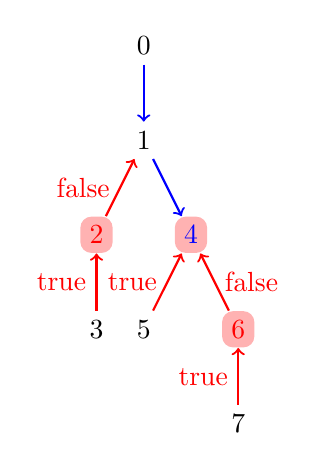
\begin{tikzpicture}
       \tikzstyle{level 1}=[level distance=1.2cm, sibling distance=1.2cm]
       \tikzstyle{childnode}=[rounded corners, black]
       \tikzstyle{marknode}=[fill=red!30, rounded corners]
       \tikzstyle{edge from parent}=[draw,thick]
       \node {0} 
        child[blue, ->] {node[childnode] {1} 
         child[red, <-] {node[marknode] {\Cb{2}}
          child {node[childnode] {3}
           edge from parent node[left] {true}
          }
          edge from parent node[left] {false}
         }
         child {node[marknode] {\Cb{4}}
          child[red, <-] {node[childnode] {5}
           edge from parent node[left] {true}
          }
          child[red, <-] {node[marknode] {\Cb{6}} 
           child {node[childnode] {7}
            edge from parent node[left] {true}
           }
           edge from parent node[right] {false}
          }
         }
        };
      \end{tikzpicture}
      }\only<17>{
      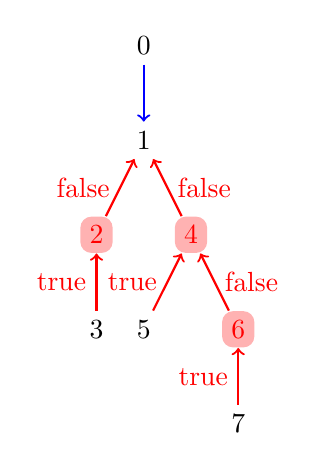
\begin{tikzpicture}
       \tikzstyle{level 1}=[level distance=1.2cm, sibling distance=1.2cm]
       \tikzstyle{childnode}=[rounded corners, black]
       \tikzstyle{marknode}=[fill=red!30, rounded corners]
       \tikzstyle{edge from parent}=[draw,thick]
       \node {0} 
        child[blue, ->] {node[childnode] {1} 
         child[red, <-] {node[marknode] {\Cb{2}}
          child {node[childnode] {3}
           edge from parent node[left] {true}
          }
          edge from parent node[left] {false}
         }
         child[red, <-] {node[marknode] {\Cb{4}}
          child {node[childnode] {5}
           edge from parent node[left] {true}
          }
          child {node[marknode] {\Cb{6}} 
           child {node[childnode] {7}
            edge from parent node[left] {true}
           }
           edge from parent node[right] {false}
          }
          edge from parent node[right] {false}
         }
        };
      \end{tikzpicture}
      }\only<18>{
      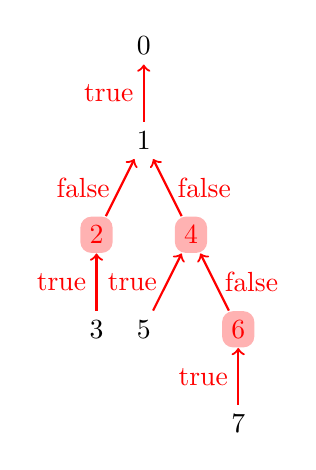
\begin{tikzpicture}
       \tikzstyle{level 1}=[level distance=1.2cm, sibling distance=1.2cm]
       \tikzstyle{childnode}=[rounded corners, black]
       \tikzstyle{marknode}=[fill=red!30, rounded corners]
       \tikzstyle{edge from parent}=[draw,thick]
       \node {0} 
        child[red, <-] {node[childnode] {1} 
         child {node[marknode] {\Cb{2}}
          child {node[childnode] {3}
           edge from parent node[left] {true}
          }
          edge from parent node[left] {false}
         }
         child {node[marknode] {\Cb{4}}
          child {node[childnode] {5}
           edge from parent node[left] {true}
          }
          child {node[marknode] {\Cb{6}} 
           child {node[childnode] {7}
            edge from parent node[left] {true}
           }
           edge from parent node[right] {false}
          }
          edge from parent node[right] {false}
         }
         edge from parent node[left] {true}
        };
      \end{tikzpicture}
      }\only<19->{
      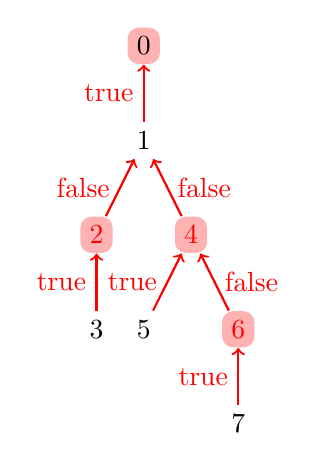
\begin{tikzpicture}
       \tikzstyle{level 1}=[level distance=1.2cm, sibling distance=1.2cm]
       \tikzstyle{childnode}=[rounded corners, black]
       \tikzstyle{marknode}=[fill=red!30, rounded corners]
       \tikzstyle{edge from parent}=[draw,thick]
       \node[marknode] {\Cb{0}} 
        child[red, <-] {node[childnode] {1} 
         child {node[marknode] {\Cb{2}}
          child {node[childnode] {3}
           edge from parent node[left] {true}
          }
          edge from parent node[left] {false}
         }
         child {node[marknode] {\Cb{4}}
          child {node[childnode] {5}
           edge from parent node[left] {true}
          }
          child {node[marknode] {\Cb{6}} 
           child {node[childnode] {7}
            edge from parent node[left] {true}
           }
           edge from parent node[right] {false}
          }
          edge from parent node[right] {false}
         }
         edge from parent node[left] {true}
        };
      \end{tikzpicture}
      }
     \end{figure}
     \only<20>{Couverture minimale = \{0,2,4,6\}}
    \end{center}
   \end{block}
  \end{frame}
